%Version 2.1 April 2023
% See section 11 of the User Manual for version history
%
%%%%%%%%%%%%%%%%%%%%%%%%%%%%%%%%%%%%%%%%%%%%%%%%%%%%%%%%%%%%%%%%%%%%%%
%%                                                                 %%
%% Please do not use \input{...} to include other tex files.       %%
%% Submit your LaTeX manuscript as one .tex document.              %%
%%                                                                 %%
%% All additional figures and files should be attached             %%
%% separately and not embedded in the \TeX\ document itself.       %%
%%                                                                 %%
%%%%%%%%%%%%%%%%%%%%%%%%%%%%%%%%%%%%%%%%%%%%%%%%%%%%%%%%%%%%%%%%%%%%%

%%\documentclass[referee,sn-basic]{sn-jnl}% referee option is meant for double line spacing

%%=======================================================%%
%% to print line numbers in the margin use lineno option %%
%%=======================================================%%

%%\documentclass[lineno,sn-basic]{sn-jnl}% Basic Springer Nature Reference Style/Chemistry Reference Style

%%======================================================%%
%% to compile with pdflatex/xelatex use pdflatex option %%
%%======================================================%%

% \documentclass[pdflatex,sn-basic,Numbered]{sn-jnl}% Basic Springer Nature Reference Style/Chemistry Reference Style


%%Note: the following reference styles support Namedate and Numbered referencing. By default the style follows the most common style. To switch between the options you can add or remove �Numbered� in the optional parenthesis. 
%%The option is available for: sn-basic.bst, sn-vancouver.bst, sn-chicago.bst, sn-mathphys.bst. %  
 
%%\documentclass[pdflatex,sn-nature]{sn-jnl}% Style for submissions to Nature Portfolio journals
\documentclass[pdflatex,sn-basic,10pt]{sn-jnl}% Basic Springer Nature Reference Style/Chemistry Reference Style
% \documentclass[pdflatex,sn-mathphys,Numbered]{sn-jnl}% Math and Physical Sciences Reference Style
%%\documentclasspdflatex,sn-aps]{sn-jnl}% American Physical Society (APS) Reference Style
%%\documentclass[pdflatex,sn-vancouver,Numbered]{sn-jnl}% Vancouver Reference Style
%%\documentclass[pdflatex,sn-apa]{sn-jnl}% APA Reference Style 
%%\documentclass[pdflatex,sn-chicago]{sn-jnl}% Chicago-based Humanities Reference Style
%%\documentclass[default]{sn-jnl}% Default
%%\documentclass[default,iicol]{sn-jnl}% Default with double column layout

%%%% Standard Packages
%%<additional latex packages if required can be included here>

\usepackage{graphicx}%
\usepackage{multirow}%
\usepackage{amsmath,amssymb,amsfonts}%
\usepackage{amsthm}%
\usepackage{mathrsfs}%
\usepackage[title]{appendix}%
\usepackage{xcolor}%
\usepackage{textcomp}%
\usepackage{manyfoot}%
\usepackage{booktabs}%
\usepackage{algorithm}%
\usepackage{algorithmicx}%
\usepackage{algpseudocode}%
\usepackage{listings}%

\usepackage{makecell}

%%%%

%%%%%=============================================================================%%%%
%%%%  Remarks: This template is provided to aid authors with the preparation
%%%%  of original research articles intended for submission to journals published 
%%%%  by Springer Nature. The guidance has been prepared in partnership with 
%%%%  production teams to conform to Springer Nature technical requirements. 
%%%%  Editorial and presentation requirements differ among journal portfolios and 
%%%%  research disciplines. You may find sections in this template are irrelevant 
%%%%  to your work and are empowered to omit any such section if allowed by the 
%%%%  journal you intend to submit to. The submission guidelines and policies 
%%%%  of the journal take precedence. A detailed User Manual is available in the 
%%%%  template package for technical guidance.
%%%%%=============================================================================%%%%

% \jyear{2023}%

%% as per the requirement new theorem styles can be included as shown below
%\theoremstyle{thmstyleone}%
\newtheorem{theorem}{Theorem}%  meant for continuous numbers
%%\newtheorem{theorem}{Theorem}[section]% meant for sectionwise numbers
%% optional argument [theorem] produces theorem numbering sequence instead of independent numbers for Proposition
\newtheorem{proposition}[theorem]{Proposition}% 
%%\newtheorem{proposition}{Proposition}% to get separate numbers for theorem and proposition etc.

%\theoremstyle{thmstyletwo}%
\newtheorem{example}{Example}%
\newtheorem{remark}{Remark}%

%\theoremstyle{thmstylethree}%
\newtheorem{definition}{Definition}%

\raggedbottom
%%\unnumbered% uncomment this for unnumbered level heads

\newcommand{\reftable}[1]{\hyperref[#1]{Table \ref*{#1}}}
\newcommand{\reffig}[1]{\hyperref[#1]{Fig. \ref*{#1}}}
\newcommand{\refsec}[1]{\hyperref[#1]{Section \ref*{#1}}}


\begin{document}

\title[MALPRED: Predictive Modeling for Malware Detection in Windows Systems using Ensemble Learning]{MALPRED: Predictive Modeling for Malware Detection in Windows Systems using Ensemble Learning}

%%=============================================================%%
%% Prefix	-> \pfx{Dr}
%% GivenName	-> \fnm{Joergen W.}
%% Particle	-> \spfx{van der} -> surname prefix
%% FamilyName	-> \sur{Ploeg}
%% Suffix	-> \sfx{IV}
%% NatureName	-> \tanm{Poet Laureate} -> Title after name
%% Degrees	-> \dgr{MSc, PhD}
%% \author*[1,2]{\pfx{Dr} \fnm{Joergen W.} \spfx{van der} \sur{Ploeg} \sfx{IV} \tanm{Poet Laureate} 
%%                 \dgr{MSc, PhD}}\email{iauthor@gmail.com}
%%=============================================================%%

%\author{Authors}

\author*[1]{\fnm{Le Qi} \sur{Yau}}\email{yau\_le\_qi@temasekjc.moe.edu.sg}
\author*[2]{\fnm{Mahir Hitesh} \sur{Shah}}\email{mahirshah2807@gmail.com}
\author*[1]{\fnm{Eugene Jin Yew} \sur{Ang}}\email{ang\_jin\_yew\_eugene@temasekjc.moe.edu.sg}
\author*[1]{\fnm{Dhanvine} \sur{Rameshkumar}}\email{rameshkumar\_dhanvine@temasekjc.moe.edu.sg}
\author*[3]{\fnm{Justin Suwattana} \sur{Chee}}\email{chee.justin.suwattana@dhs.edu.sg}
\author*[3]{\fnm{Yik Ting} \sur{Lam}}\email{oneytlam@gmail.com}
\author*[2]{\fnm{Prannaya} \sur{Gupta}}\email{prannayagupta@gmail.com}

\affil[1]{\orgname{Temasek Junior College}, \orgaddress{\street{22 Bedok S Rd}, \city{Singapore}, \postcode{469278}}}

\affil[2]{\orgname{NUS High School of Mathematics and Science}, \orgaddress{\street{20 Clementi Ave 1}, \city{Singapore}, \postcode{129957}}}

\affil[3]{\orgname{Dunman High School}, \orgaddress{\street{10 Tanjong Rhu Rd}, \city{Singapore}, \postcode{436895}}}

%%==================================%%
%% sample for unstructured abstract %%
%%==================================%%

\abstract{Malware infections are a pervasive issue for computers running the Windows operating system. In this study, we present a machine-learning based approach to predict the likelihood of malware infection in Windows machines. Our methodology involves conducting data pre-processing, feature engineering, and selection on the Microsoft Malware Prediction dataset. We then perform extensive experimentation using various machine learning algorithms and identify XGBoost, LightGBM and CatBoost as the 3 best-performing algorithms. Through hyperparameter tuning via the Tree-Structured Parzen Estimator and using a Meta Learner on top of our top 3 best-performing algorithms, our optimal novel model achieves an AUC score of 73.24\% across Stratified 5-fold cross-validation, demonstrating the efficacy of our approach.}

\keywords{Machine Learning, Windows, Tree-Structured Parzen Estimator, Stacked Metalearner, Gradient Boosting}

%%\pacs[JEL Classification]{D8, H51}

%%\pacs[MSC Classification]{35A01, 65L10, 65L12, 65L20, 65L70}

\maketitle

\section{Introduction}\label{sec:sec-intro}

The Microsoft Windows Operating System (hereby referred to as Windows OS) is one of the most widely-used operating systems in the world, with more than 1.4 billion monthly active devices and 74\% of computer users running the newer versions such as Windows 10 and Windows 11 (\cite{microsoftahaha}).

The widespread use of Windows OS has led to the development of malicious software know commonly as malware that is created specifically to attack the system. A recent example is WannaCry (\cite{trautman2018wannacry}), a form of ransomware infecting 230,000 computers in the matter of hours, leading to up to \$4 billion dollars of damage.

The need for a reliable mechanism to advise users of the susceptibility of a machine to potential attack or infection, so that countermeasures can be implemented to prevent malware from causing any significant issues, is hence of utmost importance.

In this work, we analyse the specifications of a Windows OS machine to determine the likelihood of malware infection. We prepare a comprehensive set of experiments using various machine learning algorithms to find an appropriate model for usage. We then utilise a stacked metalearner architecture to learn from the best-performing models and tune them using a Tree-Structure Parzen Estimator (TPE) not investigated in prior literature.


\section{Related Works}\label{sec:related-works}

Prior to conducting our experiments, it is important to analyse the work previously done in this domain. Past works largely utilised the Microsoft Malware Prediction Dataset (\cite{microsoft-malware-prediction}), which is openly available on Kaggle. To evaluate their work, most prior work used the area under the receiving operator characteristic curve (ROC), which is hereby referred to as the AUC score.

\cite{iop2020} first preprocessed the aforementioned dataset to reduce the memory occupied by the dataset. This was done via the removal of columns that contained a $>95\%$ proportion of null samples, switching several data types to less precise forms and converting several ordinal fields into nominal fields. They then used Chi-square testing to filter out categorical labels not having a significant importance on the label. Following this extensive preprocessing, the remaining 42 columns were used to train three models: Logistic Regression, K-Nearest Neighbours (KNN) and Light Gradient Boosting Machine or LightGBM (\cite{meng2016communication,ke2017lightgbm}). The team then found that the LightGBM model attained the highest of the three with an AUC score of 0.72.

\cite{shahini2019} similarly removed null columns with a $>70\%$ proportion of null samples. The team then trained a LightGBM model and attained an AUC score of 0.74, aggregated over five folds. The team determined (using LightGBM's feature importance analysis system) that the features \texttt{CityIdentifier}, \texttt{FirmwareVersionIdentifier} and \texttt{SystemVolumeTotalCapacity} were the most contributive to their model.

\cite{bin2020analysis} performed a system of different experiments to identify a suitable model. The team trained a LightGBM with 5-fold cross validation and acquired an AUC score of 0.73232. They also performed a separate analysis where they converted the dataset into a sparse matrix to be utilised more effectively in memory. They used a LightGBM Baseline model for their work and attained an AUC score of 0.73926. The team also tested their methodology with a Decision Tree Classifier and Neural Network to limited success in performance.

\cite{bakanov2021development} performed a removal of columns that contained a $>90\%$ proportion of null samples, then proceeded to perform similar methods to \cite{iop2020}. They trained a LightGBM and CatBoost model achieving AUC scores of 0.74064 and 0.73557. The team also later developed a web application to interface with the LightGBM model (as it performed the best of the two) trained using the Python Eel web development framework.

The general results found in prior literature is summarised in \reftable{tab:litreview_results}. We note that all these papers attained the best results with the LightGBM model. The model trained by \cite{bakanov2021development} achieved the largest AUC score, not accounting for separate folds, whereas the model trained by \cite{shahini2019} achieved the largest cross-validated AUC score over 5 folds.

\begin{table*}[ht]
    \centering
    \caption{Summary of Prior Literature in the field of Microsoft Malware Prediction (best results bolded)}
    \begin{tabular}{ccc}
        \toprule \textbf{Source} & \textbf{AUC score} & \textbf{k-Folded?} \\
        \midrule \cite{iop2020} & 72.00\% &  \\
        \cite{shahini2019} & \textbf{74.00\%} & \checkmark \\
        \cite{bin2020analysis} & 73.23\% & \checkmark \\
        \cite{bakanov2021development} & \textbf{74.06\%} & \\
        \bottomrule
    \end{tabular}
    \label{tab:litreview_results}
\end{table*}

\section{Methodology}\label{sec:methodology}

\begin{figure}[ht]
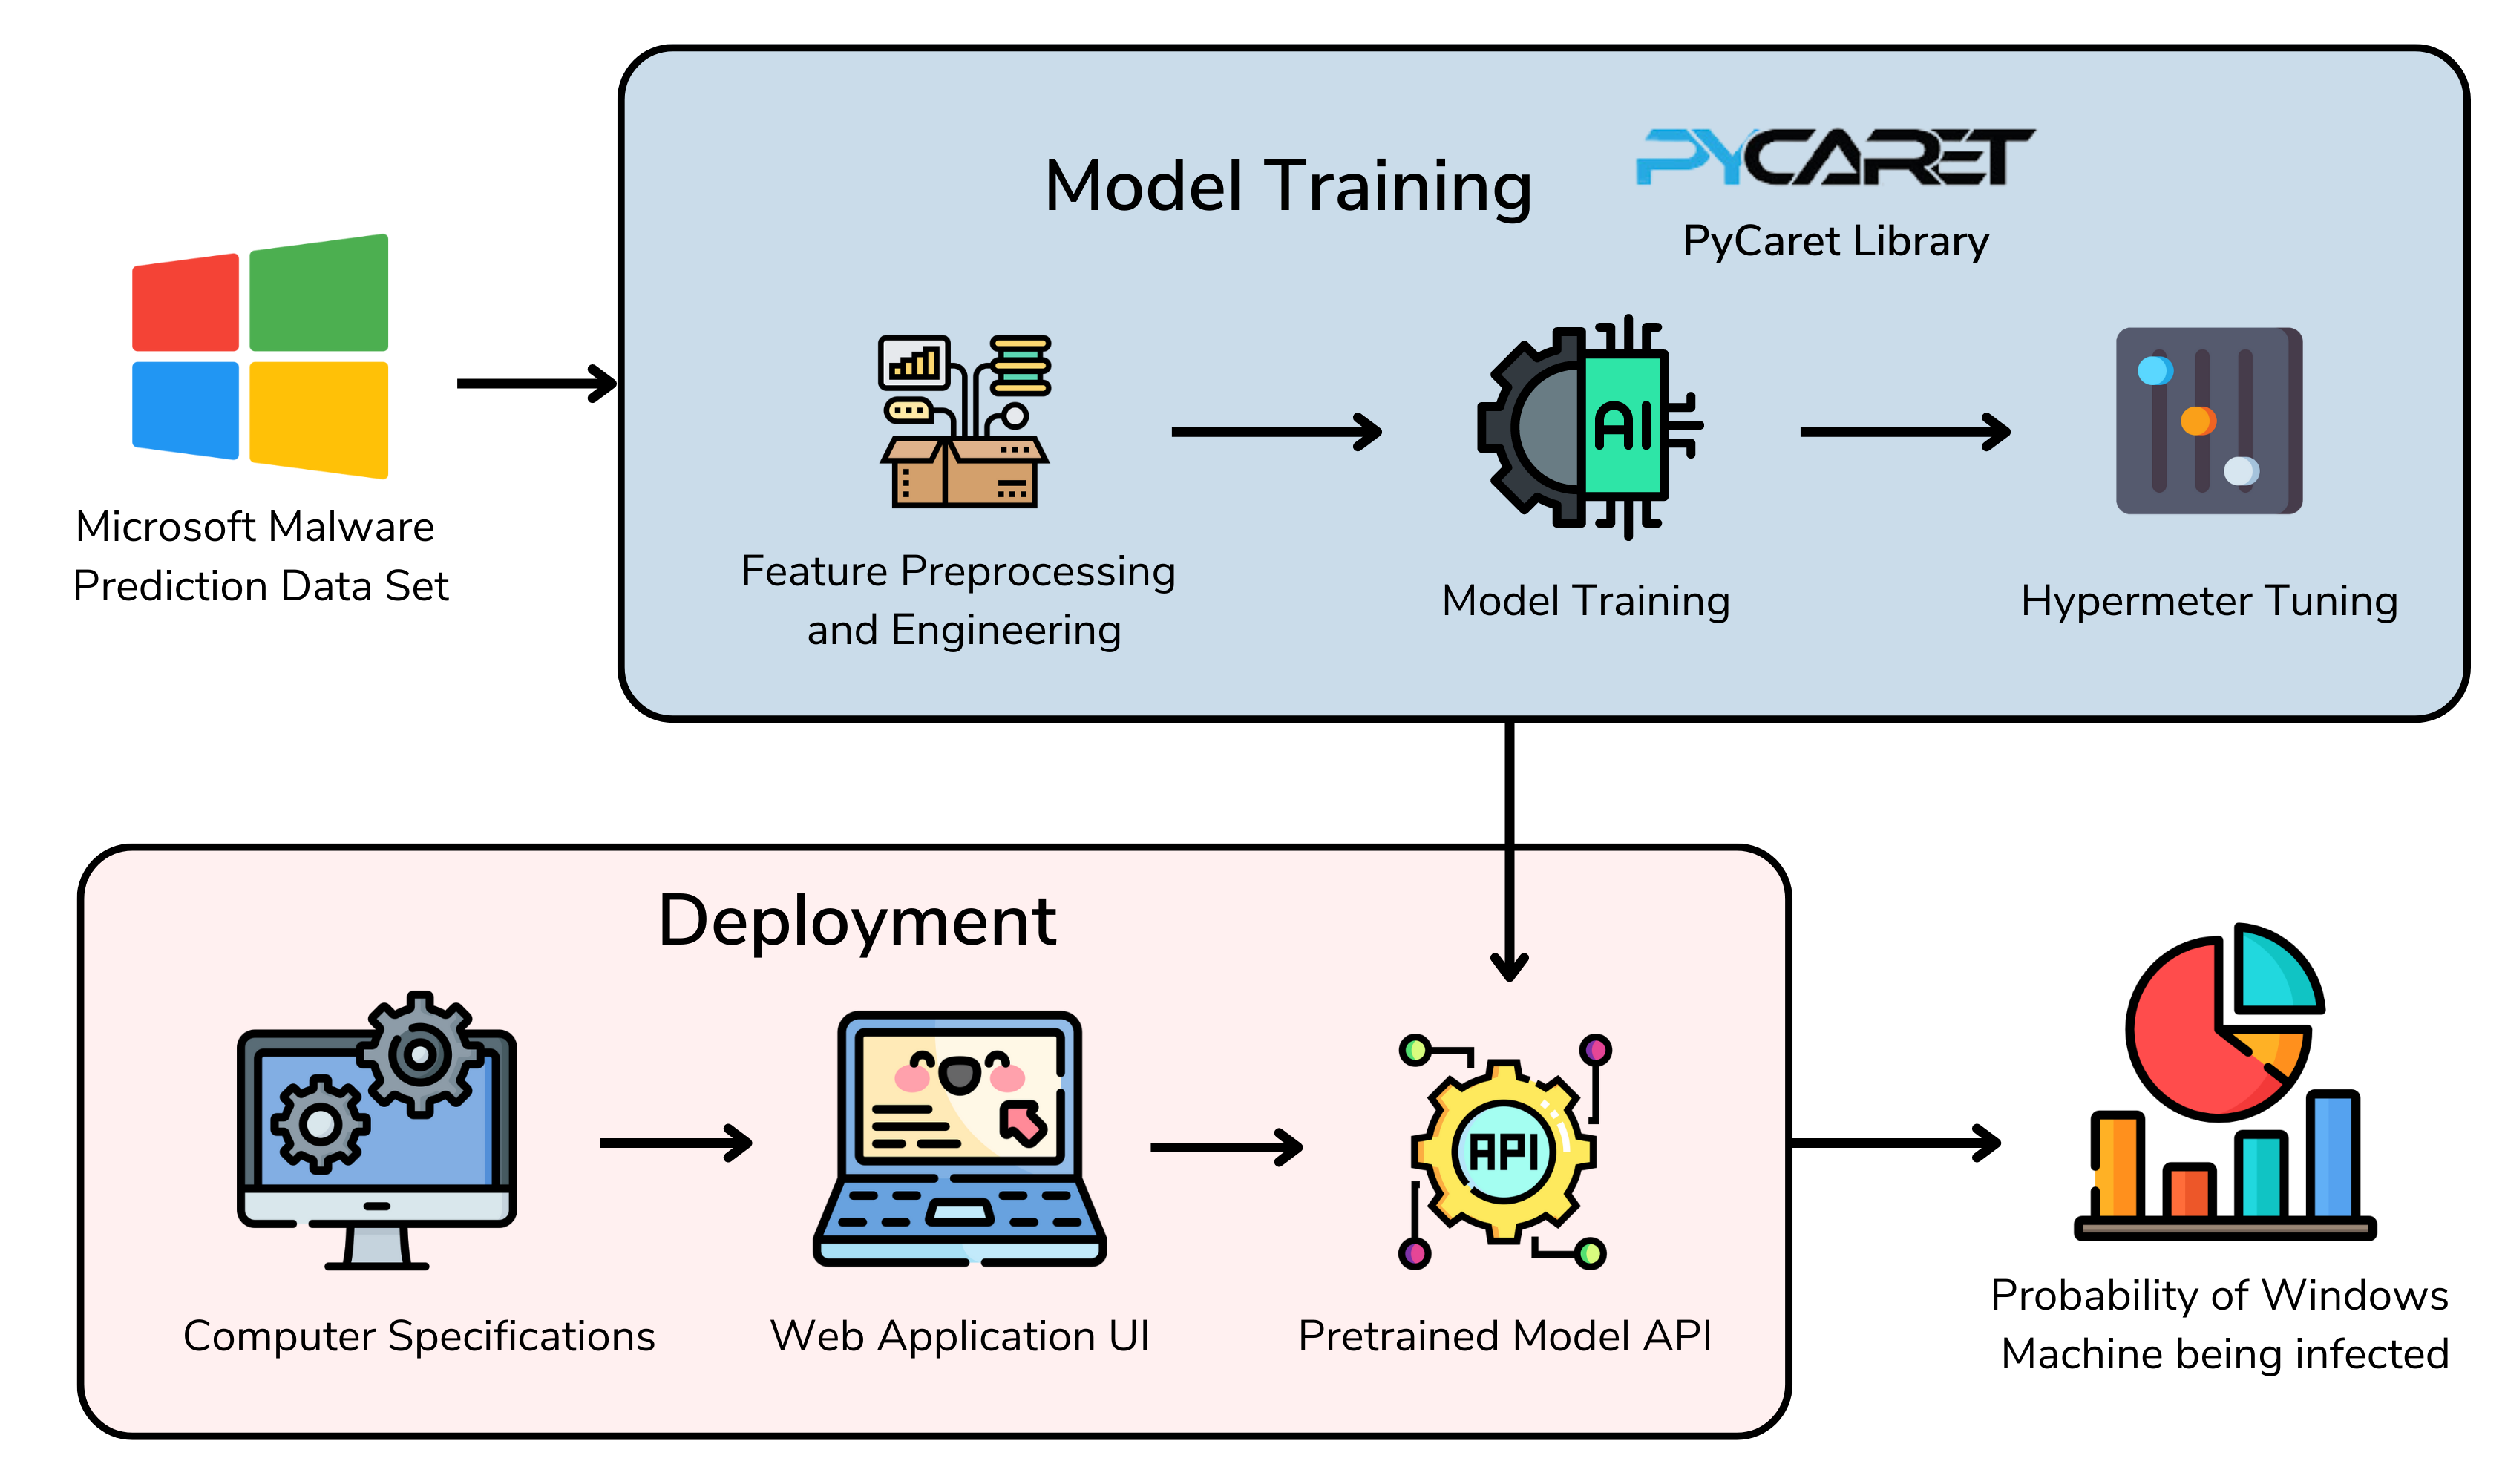
\includegraphics[width=0.8\textwidth]{images/mmp_diagram}
\centering
\caption{A simple overview of our approach}
\label{fig:fig-1}
\end{figure}

\reffig{fig:fig-1}\footnote[1]{Icons from Pixel Perfect, Eucalyp, Paul J., Freepik, and Canva have been used when designing the figures.} presents an overview of our methodology. Our methodology is split into 2 major phases.

The first phase involves the training and tuning of several models on the aforementioned Microsoft Malware Prediction dataset (\cite{microsoft-malware-prediction}). Here, we perform extensive feature preprocessing and engineering on the dataset, and we use the PyCaret Library (\cite{pycaret}) to train an optimal model on this dataset. Following this, we train the hypertuned model.

The second phase involves the deployment of our model onto a Web Application User Interface (UI) that allows users to input the specifications of their personal computers. Following this, inference is conducted and the probability of infection is displayed.

\subsection{Microsoft Malware Prediction Dataset}\label{subsec:microsoft-malware-prediction-dataset}

In this work, we use the Microsoft Malware Prediction Dataset as provided by \cite{microsoft-malware-prediction} (hereafter referred to as the MMP Dataset). This dataset is composed of 8,921,483 samples, each collecting information collected from different Windows Machines. The dataset was collected from threat and heartbeat reports from the Windows Defender application, extracting a total of 83 unique features to be used in training.

The \texttt{"HasDetections"} column indicates whether the Windows Machine has been previously infected by the malware.
As some features have many missing values while other features are not strongly correlated to whether a Windows Machine is likely to get infected, extensive feature preprocessing and engineering is required in order to achieve substantial results with machine learning models.

\subsection{The Feature Engineering and Preprocessing Pipeline}\label{subsec:feature-engineering-and-preprocessing}

An overview of our feature engineering and preprocessing pipeline is shown in \reffig{fig:fig-2}.

\begin{figure}[!t]
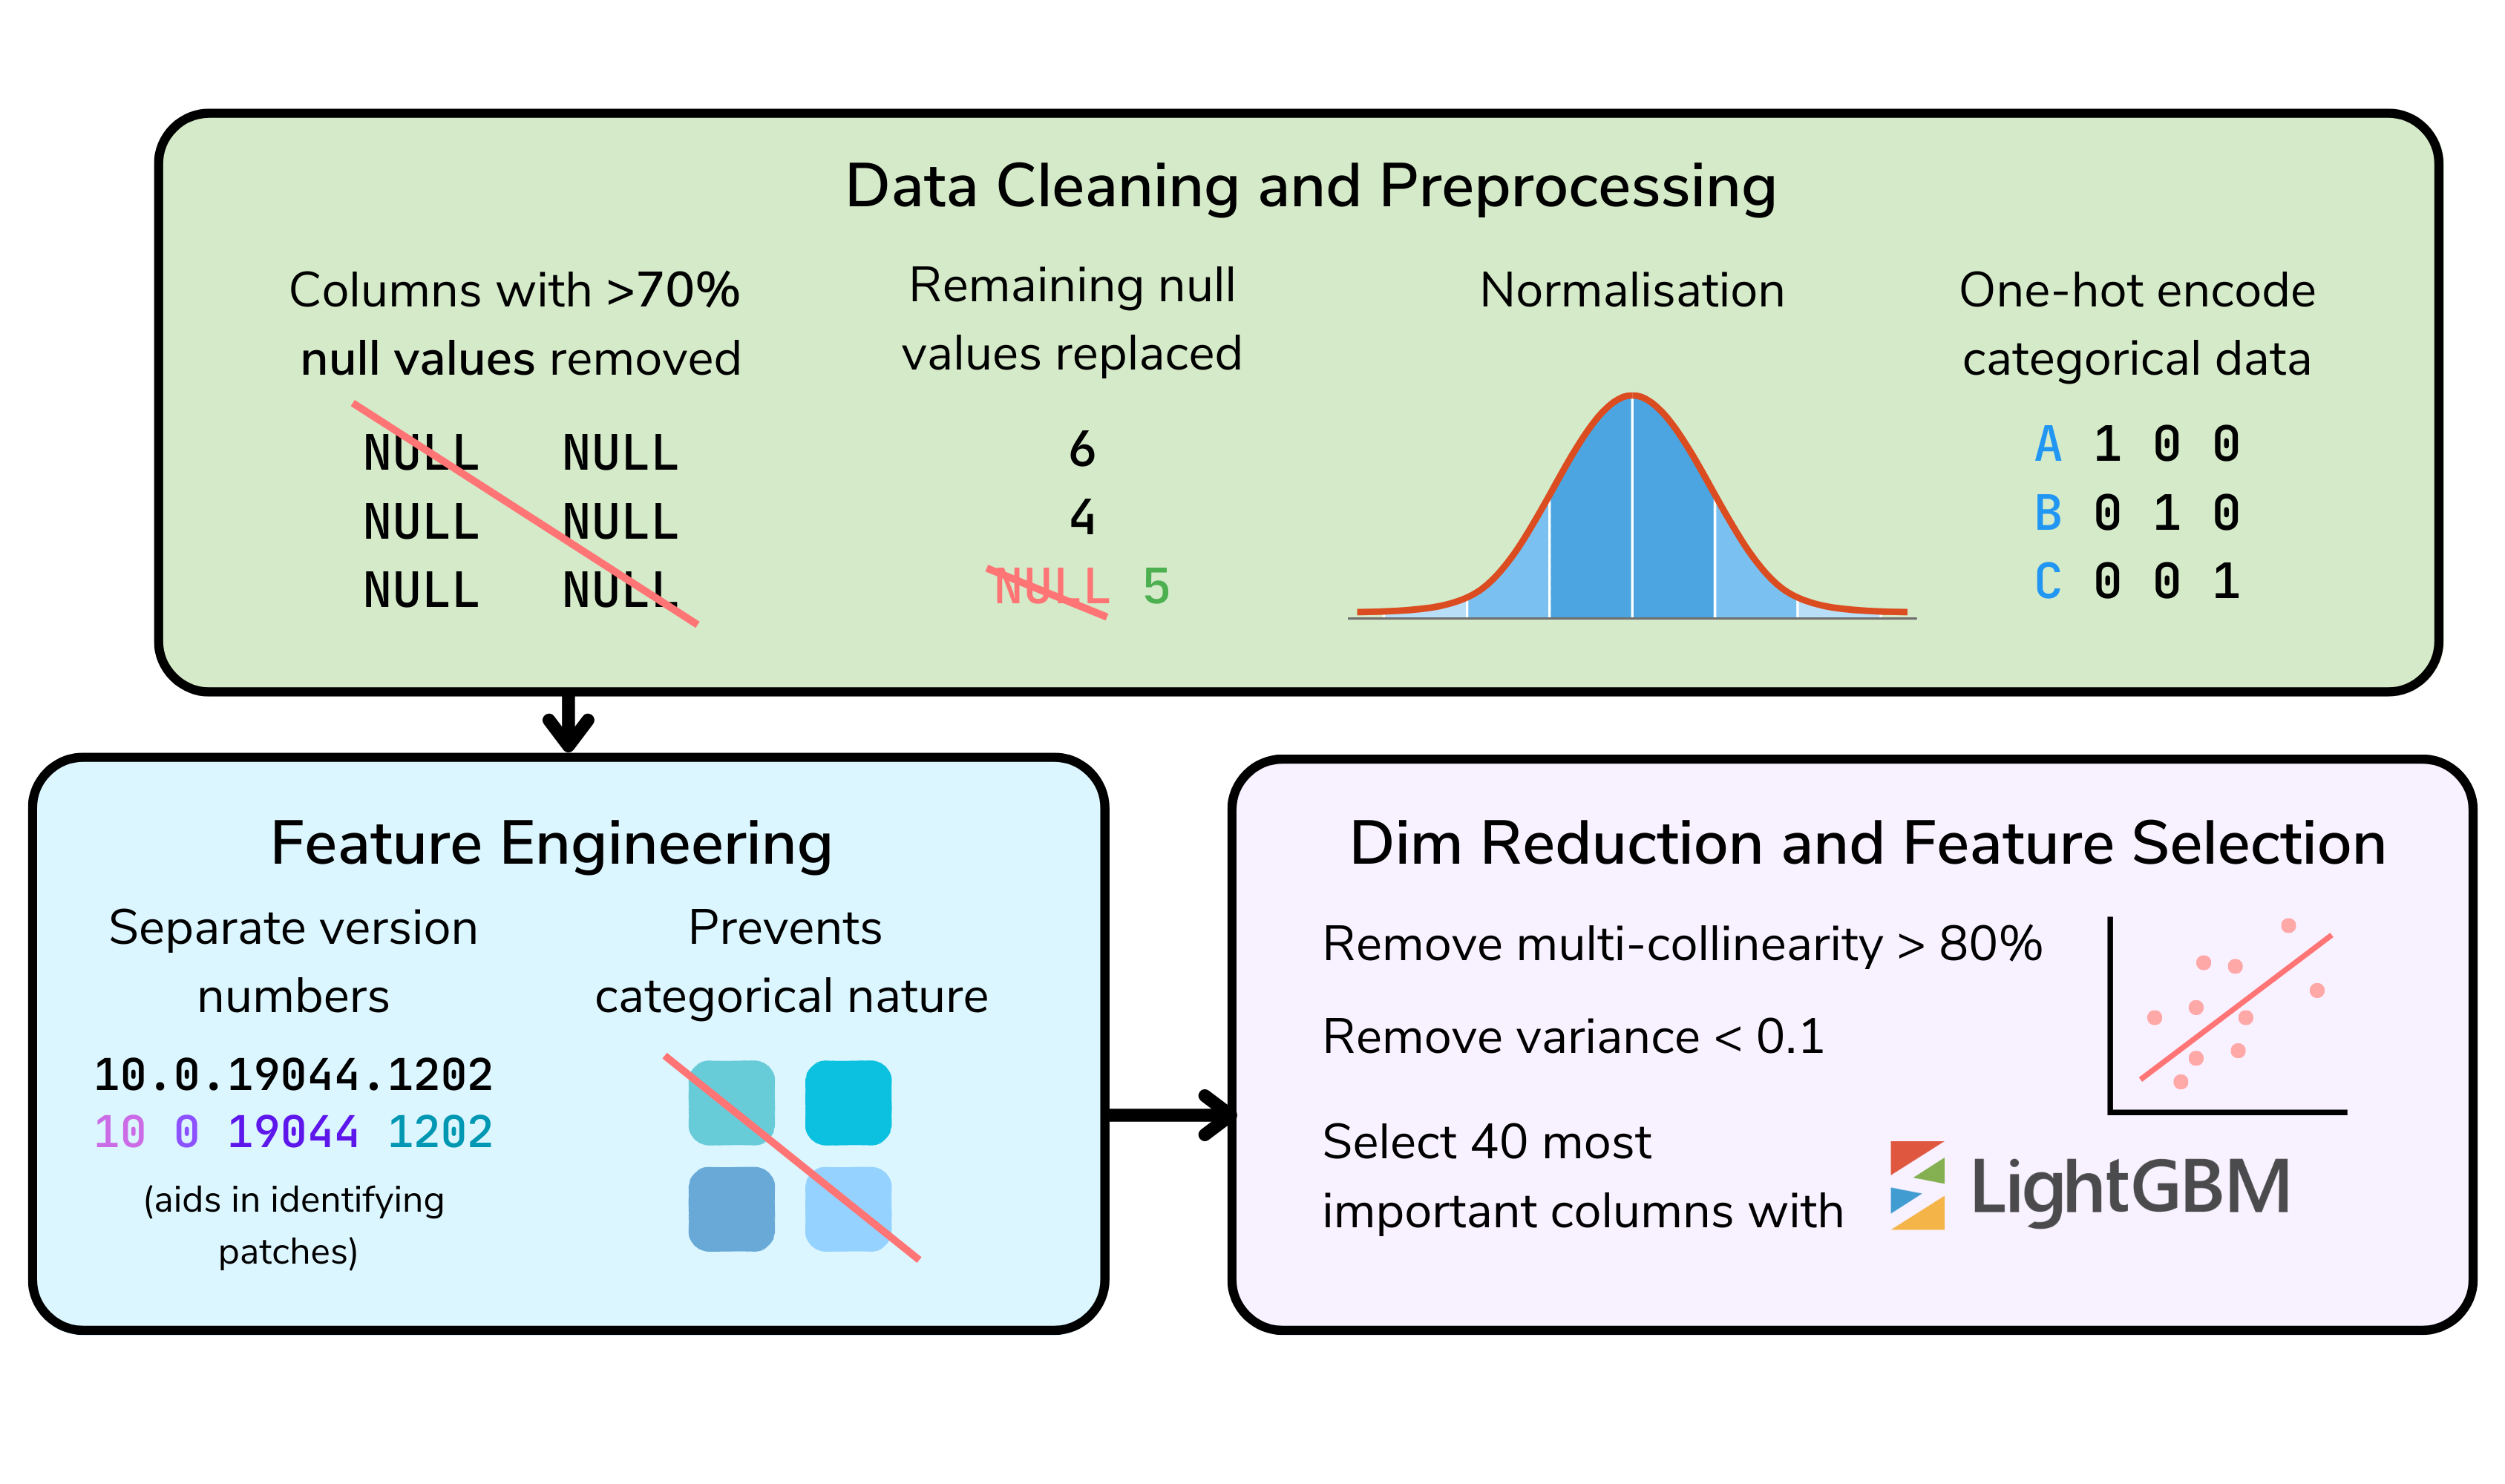
\includegraphics[width=0.8\textwidth]{images/feature_engineering}
\centering
\caption{Our Feature Engineering and Preprocessing Pipeline}
\label{fig:fig-2}
\end{figure}

\subsubsection{Data Cleaning and Processing} 
Firstly, similar to \cite{shahini2019}, columns with more than 70\% null values, {(specifically \texttt{PuaMode}, \texttt{Census
ProcessorClass}, \texttt{DefaultBrowsersIdentifier}, \texttt{Census Is FlightingInternal}, and \texttt{Census InternalBatteryType})} are noted to likely not be helpful in the task at hand and are therefore removed.
For other samples that still have null values for other columns, we utilise the simple imputer found in PyCaret to replace the null values.

\begin{itemize}
    \item For categorical columns, the null values are replaced by the most frequent value found in the column.
    \item For numerical columns, the null values are replaced by the mean of the column.
\end{itemize}

Normalisation is also performed on numeric columns such that the difference in values for all numeric columns is not drastically different. Categorical data is one hot encoded as the machine learning model is unable to process categorical data directly.

\subsubsection{Feature Engineering} 
In the provided data set, there are 6 fields which are version identifiers.
These identifiers have 4 sections separated by dots, showing the major, minor, build and patch numbers.
Since the versions that are released closer together are likely to have similar security vulnerabilities, each version field was separated such that each section is a field, similar to what is done in \cite{iop2020}.
This is to allow the models to see how close the versions are instead of having categorical data.
This can also help us find which versions may have patches for vulnerabilities.

\subsubsection{Dimension Reduction and Feature Selection}
Before we train our models, we must first investigate the dataset for any highly correlated features, as they do not generally contribute to the performance and add to the variance of the coefficients of the model.
This can lead to the model being more unstable in general, thus we remove columns where the multi-collinearity score is found to be higher than 80\%, and also columns with a variance lower than 0.1. From here, we perform Feature Selection to select the 40 most important columns using the Light Gradient Boosting Machine (LightGBM) model (\cite{meng2016communication,ke2017lightgbm}).


\subsection{Machine Learning Models}\label{subsec:machine-learning-models}
In this subsection, we introduce the various machine learning models that we used to for this task. We mainly focus on Gradient Boosted Decision Trees (GBDTs) due to their general success in modelling tabular classification tasks, as discussed in \cite{grinsztajn2022tree} and \cite{mcelfresh2023neural}.


\subsubsection{Gradient Boosting Decision Trees (GBDTs)}

\cite{friedman2001greedy} introduced the Gradient Boosting machine, a simple ensemble model that uses a set of weak learners to learn a task. This is done by incrementally training the ensemble of learners with gradient descent values. Gradient Boosting machines run iteratively over $M$ weak learners, each denoted by the value $F_m$, where $m \in \{x\in\mathbb{N}:x\leq M\}$ is the iteration number.

Gradient Boosting machines fit the first prediction, $h_0$ as a bias term to determine the mean of the expected values. This means that for a balanced dataset, $h_0 = 0.5$.

From here, for every iteration $1 \leq m \leq M$, we train a the weak learner $F_m$ to reduce the following loss function:
$$\mathcal{L}_m = J(y-h_{m-1}, F_m(x))$$
Here, the $y-h_{m-1}$ is denoted as a residual, which is used to correct the current prediction using our trained model. $J$ is a cost function, which varies depending on implementation, but for our implementation is usually the mean-squared error function.

From here, we correct the final prediction by multiplying this with a learning rate, $\alpha$ that is commonly provided. Here, $h_m = h_{m-1} + \alpha F_m(x)$. This is known as information gain as certain amount of data is added to help the estimator slowly approach the expected value. This is done until $M$, where the final prediction $h_M$ is determined.

In GBDTs, the weak learners are decision trees, a model introduced in \cite{breiman1984} and \cite{quinlan1986induction}. The decision trees split samples based on specific thresholds and conditions such that the data is partitioned properly. From here, we use the Gradient Boosting method to slowly learn the function accurately. These models have historically performed with high accuracies on several datasets and this has led to further development of models, as discussed ahead.

\subsubsection{XGBoost}
\cite{xgboost} proposed XGBoost, a Gradient Boosting Decision Tree (GBDT) model that computes both the gradients and hessians (first and second derivatives with respect to the loss) and, rather than training the weak learners on the residuals, tries to predict the ratio of the gradient and the hessian. A Taylor approximation is made to reduce the complexity of the model.
\begin{align*}
    \mathcal{L}_m &= J(y-h_{m-1}, F_m(x)) = J(y, h_{m-1}+F_m(x)) \\
    &\approx J(y, h_{m-1}) +  \frac{\partial}{\partial h_{m-1}}  \left(J(y, h_{m-1})\right) F_m (x) + \frac{\partial^2}{\partial h_{m-1}^2}  \left(J(y, h_{m-1})\right) \left[F_m (x)\right]^2
\end{align*}
Here, the first term has already been minimised in the prior iteration loop. We denote the second (gradient) term as $\mathcal{G}_{m-1}$ and the third (hessian) term as $\mathcal{H}_{m-1}$. Thus, we simplify our loss function to
$$\mathcal{L}_m = \mathcal{G}_{m-1} F_m(x) + \mathcal{H}_{m-1} \left[F_m (x)\right]^2$$
We realise that to minimize the loss function, we can define $F_m(x)$ as
$$F_m(x) = -\frac{\mathcal{G}_{m-1}}{\mathcal{H}_{m-1}}$$
Thus, we train on this value in a XGBoost iteration, rather than the original residual value. XGBoost also introduces novel features such as a sparsity-aware split-finding algorithm for the decision trees and a weighted quantile sketch for the model to scale well to larger datasets. The model also uses regularisation to prevent the model from overfitting by introducing a secondary term in our loss function.

\subsubsection{LightGBM}

Light Gradient Boosting Machine, or LightGBM, is a by-design lightweight GBDT model introduced by \cite{meng2016communication} and \cite{ke2017lightgbm}. LightGBM mostly utilises the original GBDT architecture but introduces Gradient-based One Side Sampling (GOSS) and Exclusive Feature Bundling (EFB). 

GOSS is a simple method that removes data samples that are easy to fit on, so that they do not misclassify the model as well-performing. This is done by keeping those samples that produce high gradient values while only keeping and amplifying a random sample of the data samples that produce low gradient values. This allows more focus to be placed on the underrepresented samples that produce high gradients. 

EFB, on the other hand, is a feature aggregation and selection algorithm that bundles similar features together that produce largely sparse data. This includes exclusive features such as one-hot encoded labels that take up a large amount of space, especially with a large number of zero values. EFB effectively aggregates and bundles them in order to reduce the dimensionality and speed up the training process.

Due to the extensive research done in the domain of LightGBMs since their conception, \cite{zhang2017gpu} has found a method to run LightGBM models on Graphic Processing Units (GPUs) which dynamically increase the training speed of these modules.

\subsubsection{CatBoost}

\cite{catboost} introduced categorical boosting, or CatBoost, which is another GBDT model that is able to learn over categorical data without needing one-hot encoding. This model reduces the complexity of the dataset and allows it to train much faster compared to other models that require one-hot encoded labels. CatBoost also utilises an algorithm known as symmetric weighted quantile sketch (SWQS) which handles missing values in order to reduce overfitting of any kind. This creates a symmetric tree, and this also allows faster execution. In addition, similar to XGBoost, CatBoost also makes use of the second order Taylor approximation that allows it to process more data.



\subsubsection{Other Models}

We test these GBDT models against a set of baseline models to analyse the effectiveness of the GBDT architecture over the MMP task. We analyse baselines such as the Support Vector Machine (SVM, \cite{cortes1995support}), the Decision Tree (DT, \cite{breiman1984,quinlan1986induction}), Linear Discriminant Analysis (LDA, \cite{fisher1936use}), the Multilayer Perceptron (MLP), AdaBoost (\cite{freund1995desicion}), Quadratic Discriminant Analysis (QDA, \cite{fisher1936use}) and the Ridge Classifier (\cite{horel1962application}). We also use a simplified form of a GBDT, without any major changes as proposed by XGBoost, LightGBM and CatBoost, called GBC. We also implement a Dummy classifier that ignores input features, so as to compare our trained models against a general baseline.


\subsection{Stacked Meta-Learner Model}

First introduced in \cite{rice1976algorithm}, meta learners \cite{lemke2015metalearning} are models that learn how other models are learning based on metadata. This allows it to improve the performance of an existing set of models. This also improves the flexibility of the model and reduces risks of inductive biases. Gradient boosting algorithms, for instance, fall into the general paradigm of meta-learner models.

A stacked meta-learner relies on the concept of stacked generalisation (\cite{wolpert1992stacked}), where the outputs of a set of base learners are used to deduce biases within each of these estimators. This is in order to identify which models work better together for which samples.

A meta learner composes of $M$ base learners, each denoted by the value $F_m$, where $m \in \{x \in \mathbb{N}; x \leq M\}$ is the model number. We first train each model with the loss function $\mathcal{L}_m = J(x, y)$. We then compose a feature vector of the output $F_m(x)$ values as follows:

$$h_\text{stacked} = \begin{bmatrix}
    F_1(x) \\ F_2(x) \\ \vdots \\ F_M(x)
\end{bmatrix}$$

From here, we train a meta learner model, hereby referred to as $\mathcal{M}(h)$, which takes in this stacked hypothesis output. $\mathcal{M}$ is trained over the dataset $(h_\text{stacked}, y)$. This is in order to simply figure out which results to amplify for specific stages of the system. This is effectively similar to an ensemble model.

Traditionally, stacked meta-learners use logistic regression models for $\mathcal{M}$ as they are very simple and easy to implement. In our research, we replace this logistic regression model with a XGBoost model to learn the outputs of the three best-performing models. This allows us to train a more powerful model that uses the knowledge of all three models to make its decisions.

\subsection{Tree-Structured Parzen Estimator (TPE)}\label{subsec:hyperparameter-tuning}

We use the Tree-Strucutred Parzen Estimator (TPE, \cite{bergstra2011algorithms}) to tune the hyperparameters of the best-performing set of models. This method is able to exploit the inherent tree structure of models using Decision Trees as base learners such as GBDTs. TPE balances exploration and exploitation and efficiently handles high-dimensional search spaces using Parzen Estimators (also known as Kernel Density Estimators) to reduce computational resources in retraining several models.

\section{Results}\label{sec:results}

\subsection{Feature Importance}\label{subsec:feature-importance}

\begin{figure}[!ht]
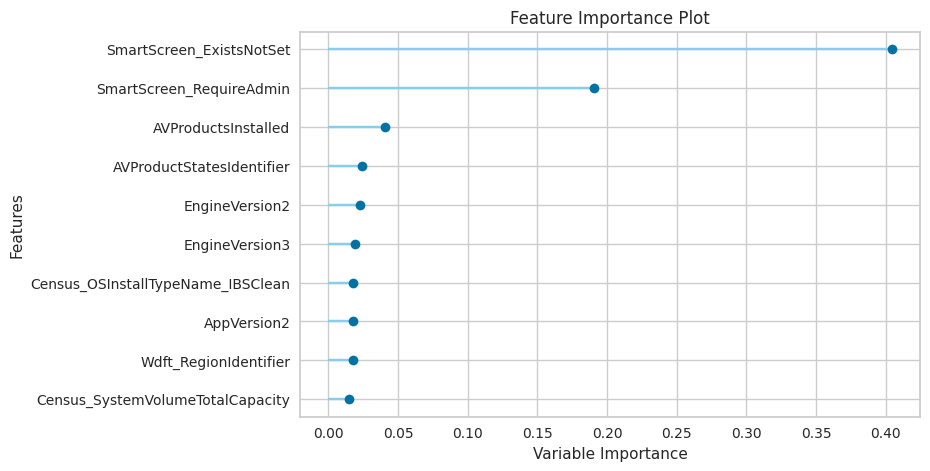
\includegraphics[scale=0.5]{images/importance}
\centering
\caption{Feature Importance of Top 10 fields}
\label{fig:fig-3}
\end{figure}

Before we begin experimenting, it is necessary to identify which features play the biggest role in the decisions of the model to see what improvements can be made to decrease the susceptibility of malware attack on specific devices. We use LightGBM's (\cite{meng2016communication,ke2017lightgbm}) built-in feature importance method to identify this result.

As seen in \reffig{fig:fig-3}, features related to the Smart Screen and the Anti-Virus, which are Windows systems that are built to protect computers from getting infected, appear highest and have a large amount of importance to the model.

\subsection{Experimental Setup and Metrics}\label{subsec:experimental-setup-and-metrics}

We evaluate the models using 5-Fold Cross Validation, where the dataset is split into 5 equal sets, and four sets are used for training the model, while one set is used for the evaluation of the model. The process is repeated until all 5 sets of data have been tested individually and the scores for each fold will be averaged. This allows us to test the entire dataset properly on the model of our choice and reduce any bias incurring from just using a specific test set.

To evaluate our models' performance, we use the AUC score, Accuracy, Recall and Precision. To identify the best performing models, we use the AUC score as the focus of the classifier is generating the probabilities of malware infections. This also makes it consistent with \cite{microsoft-malware-prediction} which used AUC score as the main metric of analysis.


\subsection{Experiments with Machine Learning Models}\label{subsec:experiments-with-machine-learning-models}
After training all the models, we identify that the XGBoost, LightGBM and CatBoost (in that order) models perform the best on the task. Hence we create a Stacked Meta-Learner using these three models as the base learners. As shown in \reftable{tab:allaimodels}, the Stacked Meta-Learner Model outperforms the base learners and achieves a non-tuned AUC score of 0.7303. The Ridge and SVM models do not generate probabilities, hence they do not have AUC scores allocated.

\begin{table*}[ht]
\centering
\caption{Score of Machine Learning Models over 5-fold Cross Validation (Best results bolded)}
\label{tab:allaimodels}
\begin{tabular}{@{}lcccccc@{}}
\toprule
 \textbf{Models} & \textbf{AUC (\%)} & \textbf{Accuracy (\%)} & \textbf{Recall (\%)}  & \textbf{Precision (\%)} \\ \midrule
\textbf{Meta-Learner} & \textbf{73.03} & \textbf{66.45} & \textbf{66.25} & \textbf{66.49} \\
XGBoost & $72.19$ & $65.79$ & $65.18$ & $65.96$ \\
LightGBM & $71.25$ & $65.08$ & $64.21$ & $65.33$ \\ 
CatBoost & $70.92$ & $64.78$ & $63.50$ & $65.15$ \\ 
MLP & $70.72$ & $64.62$ & $63.56$ & $64.94$ \\ 
GBC & $69.50$ & $63.57$ & $64.22$ & $63.38$ \\ 
AdaBoost & $68.75$ & $63.14$ & $64.87$ & $62.68$ \\ 
LDA & $66.72$ & $61.68$ & $57.79$ & $62.64$ \\ 
QDA & $66.23$ & $56.98$ & $65.85$ & $61.51$ \\ 
DT & $57.60$ & $57.60$ & $57.73$ & $57.56$ \\ 
Dummy & $50.00$ & $50.02$ & $00.00$ & $00.00$ \\ 
Ridge & $-$ & $61.68$ & $57.79$ & $62.64$ \\
SVM & $-$ & $61.34$ & $51.93$ & $63.97$ \\ \bottomrule
\end{tabular}%
\vspace{-1ex}
\end{table*}

\subsection{Experiments with Hypertuning}\label{subsec:experiments-with-hypertuning}

We use the TPE algorithm to tune the XGBoost, LightGBM and CatBoost models over 100 iterations. Due to limited resources, we extract 10\% of the dataset for our tuning. As shown in \reftable{tab:hypertuning}, the tuned models for both XGBoost and CatBoost outperform the original models for AUC score. LightGBM (not included) does not outperform the original model. We then reconstruct the Stacked Meta-Learner Model using these tuned models. This model performs the best, with an AUC score of 0.7324.

\begin{table*}[ht]
\centering
\caption{Comparison of original and hypertuned models (in percentage)}
\label{tab:hypertuning}
\begin{tabular}{@{}lcccccc@{}}
\toprule
 \textbf{Models} & \textbf{AUC} & \textbf{Accuracy} & \textbf{Recall}  & \textbf{Precision} \\ \midrule
XGBoost & $72.19$ & $65.79$ & $65.18$ & $65.96$ \\ %\hline
 XGBoost (TPE Tuned) & $72.95$ & $64.95$ & $\mathbf{80.58}$ & $61.38$ \\ \hline
CatBoost & $70.92$ & $64.78$ & $63.50$ & $65.15$ \\ %\hline
 CatBoost (TPE Tuned) & $72.37$ & $65.95$ & $65.11$ & $66.20$ \\ \hline
 Stacked Model & $73.03$ & $\mathbf{66.45}$ & $66.25$ & $\mathbf{66.49}$ \\ %\hline
 Stacked (TPE Tuned) & $\mathbf{73.24}$ & $65.36$ & $79.81$ & $61.90$ \\ \bottomrule %\hline
\end{tabular}%
\vspace{-2ex}
\end{table*}

\subsection{Experiments with Other Approaches}

We test our tuned Stacked Meta-Learner Model against \cite{shahini2019}'s approach, which achieved a state-of-the-art (SoTa) cross-validated AUC score of 0.74 across five folds. We rerun their method with the same five folds as us, and our results are prresented in \reftable{tab:comparisons}. Our tuned and untuned Stacked Meta-Leaner models outperform \cite{shahini2019}'s approach, hence we have achieved state-of-the-art performance on this task.

\begin{table*}[ht]
\centering
\caption{Score of Machine Learning Models over 5-fold Cross Validation (Best results bolded)}
\label{tab:comparisons}
\begin{tabular}{@{}lcccccc@{}}
\toprule
 \textbf{Models} & \textbf{AUC} \\ \midrule
Our Approach & $\mathbf{73.24}$ \\
\cite{shahini2019}'s Approach & $72.75$ \\
 \bottomrule
\end{tabular}%
\vspace{-20pt}
\end{table*}


\subsection{Discussion of Results}\label{subsec:discussion-of-results}

As per our initial assessment, the GBDT models performed best on the dataset. In addition, the MLP model performs marginally well, suggesting the effectiveness of a potential deep learning approach. Our Stacked Meta-Learner Model performs the best amongst the untuned models, achieving an AUC score of 73.03\%.

The TPE tuning marginally improved the performance of most of our models, with an improvement of up to 1.45\% in the AUC score. The tuned Stacked Meta-Learner achieves an AUC score of 73.24\%, outperforming \cite{shahini2019}'s approach by 0.49\%, proving the effectiveness of our approach.

\section{Conclusion}\label{sec:conclusion}

We have proposed a pipeline for feature preprocessing, engineering and selection from the MMP Dataset. We have tested our pipeline using various models. We have then developed a Stacked Meta-Learner model to learn the output of the 3 best performing modles. Finally we have performed hyperparameter tuning using the TPE method. Our final method achieves an AUC score of 73.24\%, outperforming existing methods.

% \subsection{Future Works}

In future work, we wish to explore the use of Tabular Deep Learning on the MMP dataset. As stated in \cite{mcelfresh2023neural}, deep learning models are able to achieve comparable performances to GBDTs, hence it is of great interest that we explore these models in the future.

Another potential exploration could be the collection of more recent data regarding malware attack prediction as the MMP dataset dates back to 2015 and most of the devices represented use Windows 8.1, which is not in popular use anymore. More recent data can allow us to make a model capable of diagnosing a larger portion of computers, especially those being used today with newer versions like Windows 11.

\subsection*{Availability of data and material}

The MMP dataset used is freely available on Kaggle\footnote{\url{https://www.kaggle.com/competitions/microsoft-malware-prediction}}. All code used in the paper is publicly available on GitHub\footnote{\url{https://github.com/terminalai/MALPRED}}.

\subsection*{Competing Interests}
All authors certify that they have no affiliations with or involvement in any organization or entity with any financial interest or non-financial interest in the subject matter or materials discussed in this manuscript.

\subsection*{Acknowledgement}
The authors would like to acknowledge Terminal.AI\footnote{\url{https://terminalai.org/}} for its support and encouragement in this project.


\bibliography{bib}


\end{document}
